\documentclass{article}
\usepackage[utf8]{inputenc}
\usepackage{graphicx}
\title{PS6_Gao}
\author{Gaoningjing }
\date{march 2020}

\begin{document}

\maketitle

\section{Question 3}
t  
library(twitteR)
library(tm)
library(wordcloud)
library(RColorBrewer)
library(SnowballC)
library(syuzhet)
library(tidyverse)
library(tidytext)
library(ggplot2)
library(forcats)

url <- paste("https://www.infoplease.com/us/us-cities/top-50-cities-us-population-and-rank",
    sep="")
html <- read_html(url) # reading the html code into memory
html
substr(html_text(html), 1, 1000)
tab <- html_table(html)
str(tab)
city <- tab[[1]]
city
names(city)[which(names(city)=="SIZE RANK 2014")] <- "rank"
names(city)[which(names(city)=="7/1/2014POPULATION ESTIMATE")] <- "14pop"
names(city)[which(names(city)=="7/1/2013POPULATION ESTIMATE")] <- "13pop"
names(city)[which(names(city)=="4/1/2010CENSUS POPULATION")] <- "10pop"
names(city)[which(names(city)=="7/1/2005POPULATION ESTIMATE")] <- "05pop"
names(city)[which(names(city)=="4/1/2000CENSUS POPULATION")] <- "00pop"
names(city)[which(names(city)=="4/1/1990CENSUS POPULATION")] <- "90pop"
city

\section{Question 5}
 from my graphs, i see clearly know the rank of to 50 cities for 2014. it much clearer than dataset. also, i do the top 6 cities for 2013 and 2014 population. the gap of them are clear.

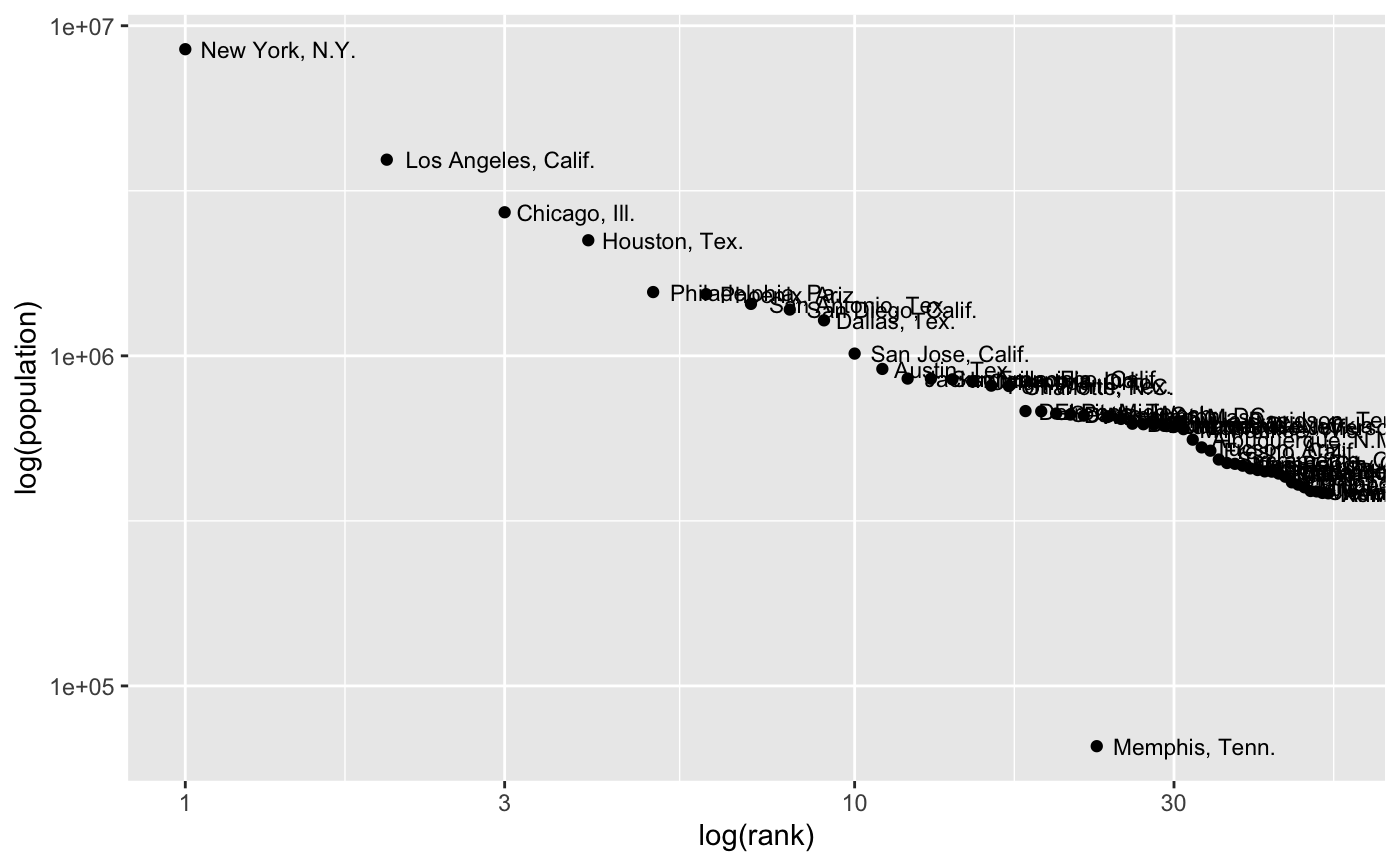
\includegraphics{PS6a_Gao.png}
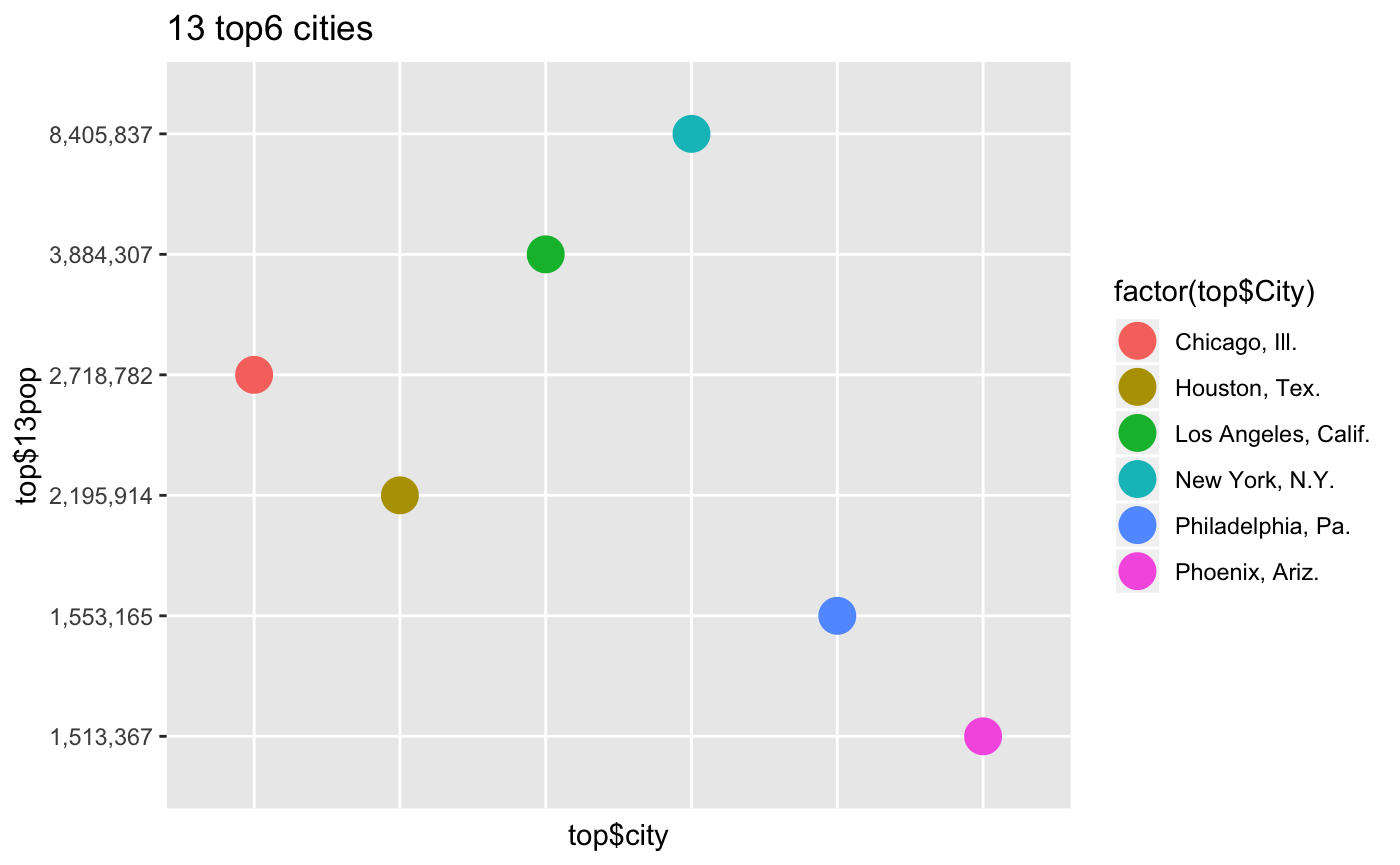
\includegraphics{PS6b_Gao.png}
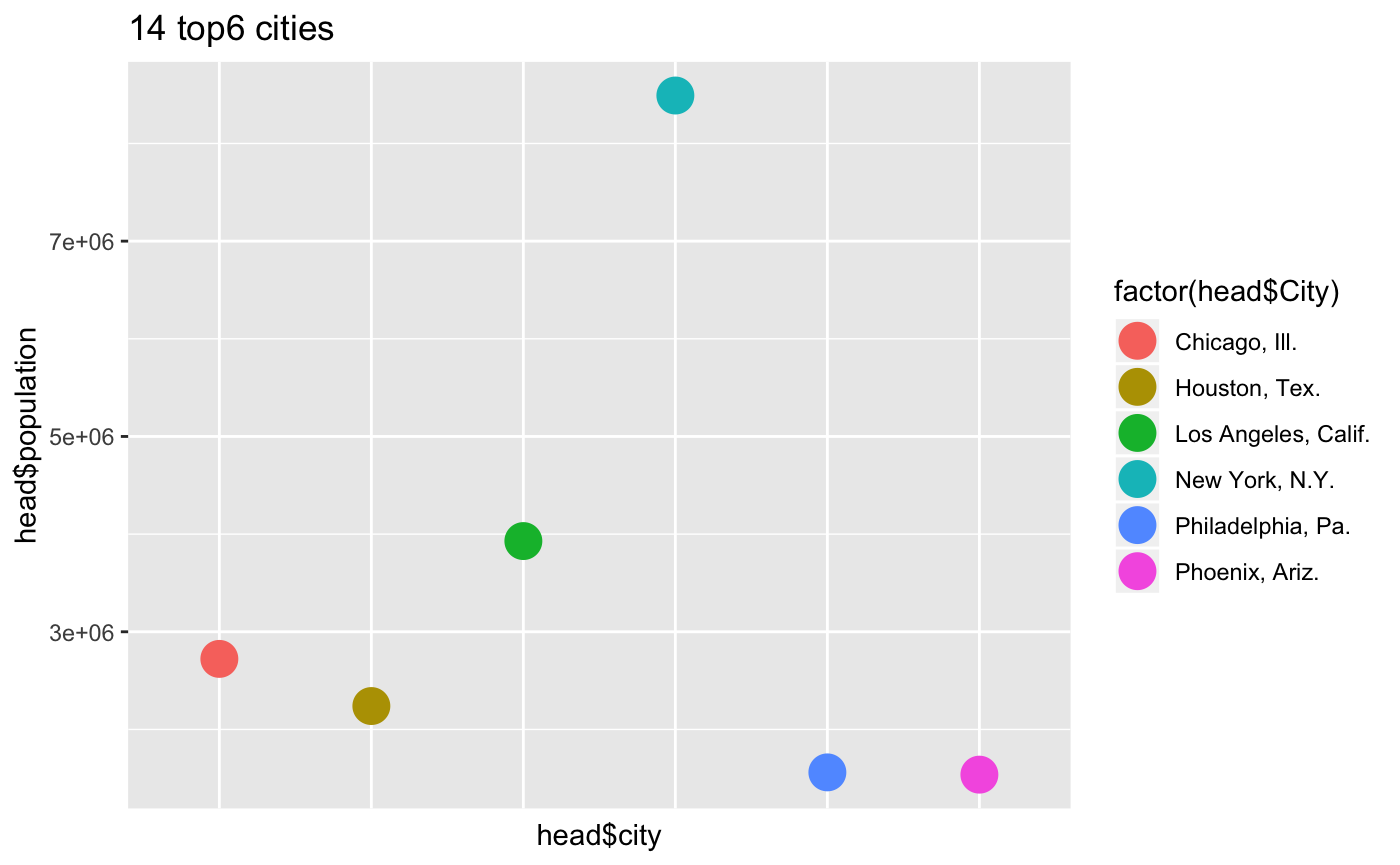
\includegraphics{PS6c_Gao.png}
\end{document}